\documentclass{kgtu}

\usepackage{amsmath,amsfonts,amssymb}
\usepackage[linesnumbered,ruled,vlined]{algorithm2e}
\usepackage{ulem} % kasim, for strikethrough
\usepackage{lipsum}

\begin{document}
\chapter{INTRODUCTION}
A doctoral thesis represents the culmination of years of rigorous research and academic pursuit. It should embody a significant contribution to the field of study, demonstrating the author's expertise and ability to conduct original research. \cite{oztoprak2023technological}An effective thesis begins with a clear and concise introduction that sets the stage for the entire work. This crucial section should provide a broad overview of the research area, gradually narrowing down to the specific problem or question being addressed. It is essential to articulate the research objectives, highlight the significance of the study, and briefly outline the methodological approach. \cite{butun2021application}The introduction should also situate the research within the existing body of knowledge, identifying gaps in current understanding that the thesis aims to fill. By the end of the introduction, readers should have a clear understanding of the thesis's purpose, its potential impact on the field, and the structure of the subsequent chapters. A well-crafted introduction not only engages the reader but also serves as a roadmap for the comprehensive exploration of the research topic that follows.\cite{oztoprak2023holistic}
\section{Sample Section}
This is sample section. This should have a number.
\lipsum[1-3]
\subsection{Sample Sub Section}
This is a sample sub section. This should have a number too.
\lipsum[4-5]
\subsubsection{Sample Subsub Section}
This is a sample sub sub section. This should not have a number too.
\lipsum[6-7]
\chapter{BACKGROUND}

This is a sample long table. In this \ref{tab:sample_longtable}, it will continue on next page.
\begin{raggedright}
\begin{footnotesize}
\begin{longtable}{{p{0.47\linewidth} p{0.22\linewidth} p{0.22\linewidth}}}
\caption{Comprehensive Research Topics in Computer Science}
\label{tab:sample_longtable}\\
\hline
\textbf{Research Topic} & \textbf{Key Methods} & \textbf{Challenges} \\
\hline
\endfirsthead

\caption[]{Comprehensive Research Topics in Computer Science (Continued)}\\
\hline
\textbf{Research Topic} & \textbf{Key Methods} & \textbf{Challenges} \\
\hline
\endhead

Artificial Intelligence in Healthcare & Machine Learning, Neural Networks & Data privacy, Model interpretability \\

Quantum Computing Algorithms & Quantum circuits, Shor's algorithm & Scalability, Error correction \\

Blockchain for Supply Chain Management & Distributed ledger, Smart contracts & Energy consumption, Scalability \\

Natural Language Processing for Sentiment Analysis & Deep Learning, BERT models & Contextual understanding, Multilingual support \\

Edge Computing for IoT & Fog computing, Edge analytics & Security, Resource constraints \\

Autonomous Vehicles & Computer vision, Reinforcement learning & Safety, Ethical decision-making \\

Cybersecurity in 5G Networks & Encryption, Intrusion detection & New attack vectors, Latency requirements \\

Virtual and Augmented Reality & 3D modeling, Motion tracking & User experience, Hardware limitations \\

Big Data Analytics in Social Media & Data mining, Predictive modeling & Data volume, Real-time processing \\

Green Computing & Energy-efficient algorithms, Sustainable hardware & Performance trade-offs, Implementation costs \\

Bioinformatics and Genomic Data Analysis & Sequence alignment, Phylogenetic analysis & Data complexity, Computational efficiency \\

Cloud Computing Optimization & Virtualization, Load balancing & Resource allocation, Data sovereignty \\

Human-Computer Interaction & User interface design, Usability testing & Accessibility, Cross-cultural design \\

Robotic Process Automation & Workflow analysis, Intelligent automation & Process complexity, Integration challenges \\

Computer Vision for Medical Imaging & Image segmentation, Pattern recognition & Accuracy, Interpretability \\

Distributed Systems for Big Data & MapReduce, Distributed file systems & Fault tolerance, Network latency \\

Artificial General Intelligence & Cognitive architectures, Transfer learning & Ethical concerns, Unpredictability \\

Quantum Cryptography & Quantum key distribution, Entanglement & Implementation costs, Key rate limitations \\

Internet of Things (IoT) Security & Device authentication, Secure protocols & Device heterogeneity, Limited resources \\

Explainable AI (XAI) & Layer-wise relevance propagation, SHAP values & Model complexity, Human comprehension \\

Federated Learning & Decentralized ML, Secure aggregation & Communication overhead, Model convergence \\

Software-Defined Networking & Network virtualization, Programmable switches & Backward compatibility, Controller scalability \\

Neuromorphic Computing & Spiking neural networks, Memristive devices & Hardware design, Algorithm adaptation \\

Privacy-Preserving Machine Learning & Differential privacy, Homomorphic encryption & Utility-privacy trade-off, Computational overhead \\

Serverless Computing & Function-as-a-Service, Event-driven architecture & Cold start latency, State management \\

Swarm Intelligence & Particle swarm optimization, Ant colony algorithms & Parameter tuning, Local optima \\

Adversarial Machine Learning & Generative adversarial networks, Robust optimization & Attack detection, Model resilience \\

Quantum Machine Learning & Quantum neural networks, Quantum support vector machines & Quantum hardware limitations, Algorithm design \\

Ethics in AI & Fairness-aware ML, Bias detection & Defining fairness, Balancing competing objectives \\

High-Performance Computing & Parallel processing, GPU acceleration & Power consumption, Algorithm parallelization \\

\hline
\end{longtable}
\end{footnotesize}
\end{raggedright}
\lipsum[8-12]
\chapter{METHODS}
\lipsum[13-15]
\chapter{EXPERIMENTAL STUDIES}
This is a sample table. You should refer it as \ref{tab:sample_table}.
Table caption will be automatically formatted.

\begin{table}[ht]
    \caption{Sample Table}
    \label{tab:sample_table}
    \begin{flushleft}
    \begin{tabularx}{\textwidth}{Xcc}  % X column adjusts width
    \toprule
    \textbf{Category} & \textbf{Item} & \textbf{Specification} \\
    \midrule
    Row 1 & Value 1A & Value 1B \\
    Row 2 & Value 2A & Value 2B \\
    \midrule
    Row 3 & Value 3A & Value 3B \\
    Row 4 & Value 4A & Value 4B \\
    Row 5 & Value 5A & Value 5B \\
    \bottomrule
    \end{tabularx}
    \end{flushleft}
\end{table}


This is a sample figure. You should refer it as \ref{fig:sample_figure}
\begin{figure}[!ht]
    \centering
    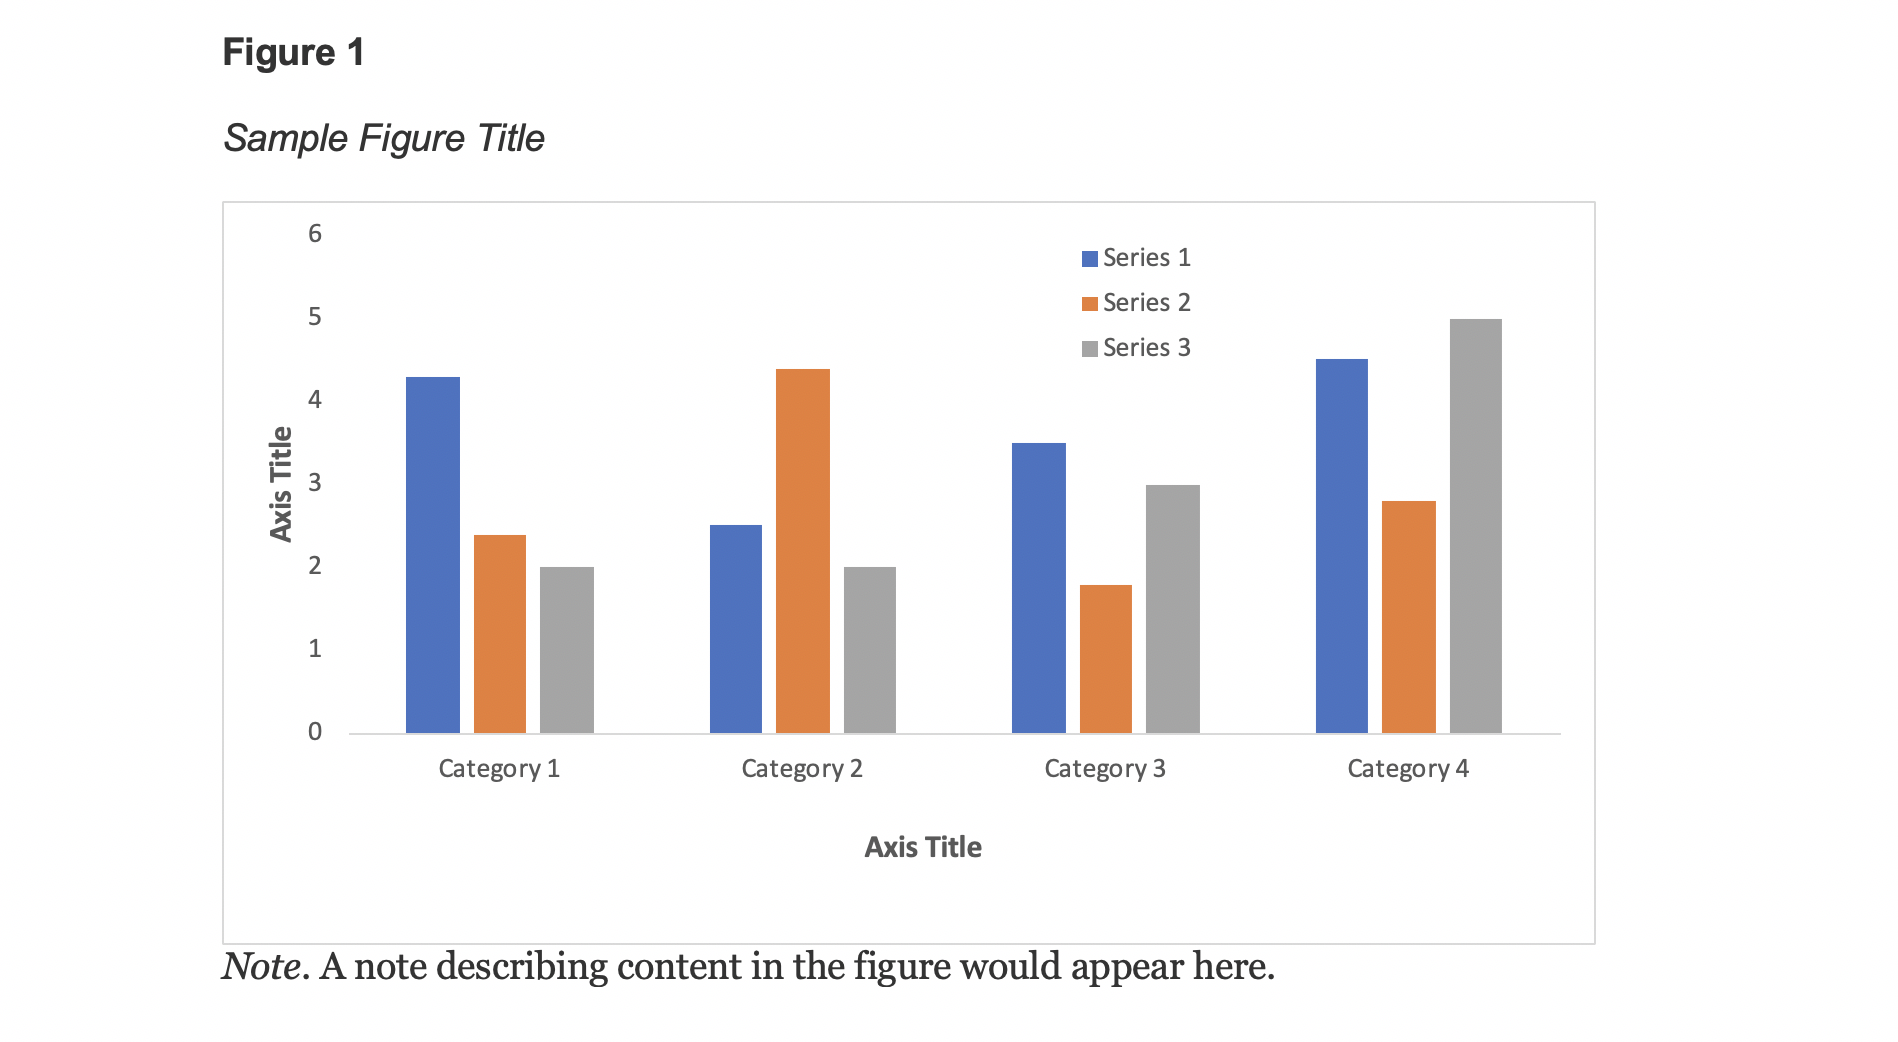
\includegraphics[width=1.0\textwidth]{figures/fig1.png}
    \caption{Sample figure showing a graph}
    \label{fig:sample_figure}
\end{figure}

This is sample algoritm. You can refer it as \ref{alg:bubblesort}.

\begin{algorithm}
\caption{Sample Algorithm: Bubble Sort}
\label{alg:bubblesort}
\KwIn{An array A of n elements}
\KwOut{Array A sorted in ascending order}
\Begin{
    \For{i = 0 to n - 1}{
        \For{j = 0 to n - i - 1}{
            \If{A[j] > A[j + 1]}{
                swap A[j] and A[j + 1]
            }
        }
    }
}
\end{algorithm}


This is a sample equation. You can refer it as \ref{eqn:quadratic}.

\begin{equation}
    \label{eqn:quadratic}
    x = \frac{-b \pm \sqrt{b^2 - 4ac}}{2a}
\end{equation}
\chapter{CONCLUSION AND FUTURE WORK}
\lipsum[15-20]

\end{document}